\section[Introduction]{Introduction}
Sentiment Analysis or Opinion Mining is a way of finding out the polarity or strength of the opinion (positive or negative) that is expressed in written text.
is used in business to understand social sentiment for their brand, a particular product or service.

\subsection[In the previous episodes]{In the previous episodes}
In the last semester, my project partner and I have for the first time stepped into the world of sentiment analysis, making use of various supports such as tutorials, explanations, and lots of research.
We then decided to use all the material we had found to build something of our own, so we tried to do a project categorizing the sentiment of hotel reviews.
We wanted to split the sentiment of the reviews into 5 categories: from awful to excellent.
At the end of the project, we managed to have an accuracy of about 0.48, taking into consideration the 5 categories was a very good result.


\subsection[Project description]{Project description}
\label{main}
The thesis project I am working on this semester, will still be on sentiment analysis, this time the model created will be used to make predictions about newspaper news, to understand the polarity of an article or the newspaper itself.
With the current rapid developments in Deep Learning, many new technologies for text analysis have emerged.
This project will make use of these technologies and develop its own "Sentiment Analysis Model".
This model can basically be imagined as a function that takes arbitrary text as input, evaluates it and classifies it into a scale of emotions from negative to positive.
To develop and train a model with this capability requires many prebuilt datasets of real examples from the Internet. These are then used to feed the model so that it can learn from these datasets and deduce correlations. Based on these correlations, the model will then be able to process arbitrary texts and assign sentiment values to them.


\subsection{Motivation}
As already mentioned, this technology allows you to crystallize negative and positive feelings from a text. Besides sentiment classification, sentiment analysis brings many other benefits in areas such as marketing and customer satisfaction. Some of these benefits could be, for example:

\begin{itemize}
\item \textbf{Customer classification}\\
Sentiment analysis allows customers to be classified according to their emotional mood. This offers the opportunity to find customers who are more willing to buy.
\item \textbf{Chatbot training}\\
With the results of the Sentiment Analysis Tool, it is possible to train chatbots to recognize and respond to specific customer sentiments.
\item \textbf{Scalability and automation}\\
As a digital tool, Sentiment Analysis can be easily extended or integrated into an automated system.
\end{itemize}

From these points, a strongly increasing tendency regarding the application of sentiment analysis can be assumed. This makes it all the more relevant for developers to get to grips with it. From the developer's perspective, learning sentiment analysis also promotes new experiences in areas such as: 

\begin{itemize}
\item Data analytics
\item Data science
\item Machine learning
\item Predictive modelling
\end{itemize}

\subsection[Goal]{Goal}
\label{main}
The core of this project is with the help of different tools like Tensorflow\cite{tensorflow}, Keras and BERT to create a "model" that takes text as input and classifies it in “positive” or “negative”. 
To calculate the polarity of the article, I will use different datasets so that I can train and test the model and see if with different datasets there different results are.
Unfortunately, due to an impediment, my partner from the previous project was not able to take part in this assignment, which means that I must continue this project alone.
For a matter of timing and difficulty, I have resized the project and the categories on which to make a prediction will no more be 5 as in the last project, but 2.
This model should be available as a single component that can be integrated into arbitrary applications.\\
For the implementation of the project, I have used several websites and tutorials:
\begin{itemize}
    \item Tutorial for Keras\cite{tutorial_keras}
    \item Deep-Learning-For-Hackers\cite{git}
    \item Sentiment Analysis with TensorFlow 2 and Keras\cite{tutorial}
    \item Deep Learning LSTM for Sentiment Analysis\cite{karikari_deep_2020}
    \item Natural Language Processing and Sentiment Analysis using Tensorflow.\cite{khan_natural_2020}
    \item Sentiment Analysis: First Steps With Python's NLTK Library - https://realpython.com/python-nltk-sentiment-analysis/
    \item Practical Text Classification With Python and Keras - https://realpython.com/python-keras-text-classification/#choosing-a-data-set
    \item Classify text with BERT - https://www.tensorflow.org/tutorials/text/classify_text_with_bert
    \item Simple Transformers — Multi-Class Text Classification with BERT, RoBERTa, XLNet, XLM, and DistilBERT - https://medium.com/swlh/simple-transformers-multi-class-text-classification-with-bert-roberta-xlnet-xlm-and-8b585000ce3a
    \item Fine-tuning BERT with Keras and tf.Module - https://towardsdatascience.com/fine-tuning-bert-with-keras-and-tf-module-ed24ea91cff2
    \item Text Classification with BERT using Transformers for long text inputs - https://medium.com/analytics-vidhya/text-classification-with-bert-using-transformers-for-long-text-inputs-f54833994dfd
    
\end{itemize}

\subsection{Project organization}
The table~\ref{tab:Organisation} describes who occupies which role in our project organization:
\begin{longtable}[ c ]{| m{5cm} | m{5cm}|  m{3cm}|}
 \hline
 \multicolumn{3}{| c |}{\textbf{Project organization}}\\
 \hline
 \textbf{Role in the \newline project organization} & \textbf{Name}  & \textbf{BFH\newline Abbreviation}\\
 \hline
 \endfirsthead
%
 \multicolumn{3}{c}%
 {{\bfseries Table \thetable\ continued from previous page}} \\
 \hline
 \textbf{Role in the \newline project organization} & \textbf{Name}  & \textbf{BFH Abbreviation}\\
 \hline
 \endhead
%
{Tutor}   & {Mascha Kurpicz-Briki}  & {kim3}   \\ \hline
{Expert}  & {Andreas Dürsteler}         & {-}   \\ \hline
{Developer}     & {Giorgio Bakhiet Derias}& {bakhg1}\\ \hline
                 
\caption{Project organization}
\label{tab:Organisation}\\
\end{longtable}
\newpage
\subsection{Tools}
In the table~\ref{tab:Tools} you can find the different tools I used for this project:
\begin{longtable}[ c ]{| m{4cm} | m{10cm}|}
 \hline
 \multicolumn{2}{| c |}{\textbf{Tools}}\\
 \hline
 \textbf{Tool}  & \textbf{Description}\\
 \hline
 \endfirsthead
%
 \multicolumn{2}{c}%
 {{\bfseries Table \thetable\ continued from previous page}} \\
 \hline
\textbf{Tool}  & \textbf{Version}\\
 \hline
 \endhead
%
{Google   \gls{colab}oratory} & {Online platform to host \gls{jupyter}.} \\ \hline
{\gls{jupyter}}           & {A document that can store code, diagrams, graphics and much more.}      \\ \hline
{\gls{anaconda}}          & {Application to manage libraries of larger projects.}      \\ \hline
{\gls{virtual machine}}   & {\gls{anaconda} is installed on the virtual machine to run the project.}      \\ \hline
{Tensorflow}   & {Open source software library for machine learning.}      \\ \hline
{\gls{keras}}             & {Tensorflow library specifically for creating neural networks.}      \\ \hline
{BERT}   & {Is a recent paper published by researchers at Google AI Language.}      \\ \hline
{\gls{Scikit-learn}}           & {Open source machine learning software library for the Python programming language.}      \\ \hline
{\gls{kaggle} (dataset)}   & {Website offering datasets and examples on Deep Learning.}      \\ \hline   
{PyCharm}   & {IDE used for the Python language. It is developed by the company JetBrains.}      \\ \hline
{GitHub}   & {GitHub is a hosting service for software projects.}      \\ \hline
{Overleaf}   & {Overleaf is a cloud-based collaborative LaTeX editor used to write, edit, and publish scientific papers.}      \\ \hline
\caption{Tools}
\label{tab:Tools}\\
\end{longtable}


\subsection{The development environment}
This section will explain all the components used for the development environment. 
\subsubsection{Jupyter Notebook}
The model is developed in the form of a \gls{jupyter} notebook using the Python programming language. \gls{jupyter} notebooks are documents that can contain code, text, images, diagrams and explanations. This is especially suitable for this project, because in Machine Learning it is often useful to explain the sourecode with graphs and diagrams.

\subsubsection{Google \gls{colab}oratory}
The notebook was initially hosted on Google \gls{colab}oratory\cite{colab}. This brought the following advantages:
\paragraph{Synchronization} 
By storing the notebook in a central location, Google Drive, and having everyone access the same notebook, all changes are immediately visible to all users of the notebook.
\paragraph{Project structure} 
The \gls{jupyter} allows to map the whole project in a structured way in a single file. 
\paragraph{Project dependencies}
Since the project is hosted on Google \gls{colab}, it is not necessary as a developer to install libraries and other dependencies locally.

However, as it turned out, \gls{colab} removes from the platform external resources that were imported into the project after a certain time. This meant that I had to re-import the datasets, which are essential for the development of my model, before each work. This forced me to set up a \gls{virtual machine} on which the notebook can then be run locally.

\subsubsection{The \gls{virtual machine}}
spiegazione vm

\subsubsection{Anaconda}
Anaconda is a distribution of the Python and R programming languages, used for data science, machine learning etc.
Anaconda is used to simplify package management and deployment of various libraries.
To run \gls{jupyter} with all the needed libraries, \gls{anaconda} has turned out to be a suitable solution. \gls{anaconda} is a platform that allows you to set up large projects locally by creating so-called "environments" that contain all the required configurations and libraries for the project. To my advantage, \gls{anaconda} already provides a pre-built environment for \gls{jupyter} projects, which is already equipped with all my needed tools, as you can see on image~\ref{fig:fig_01}.

\begin{figure}[ht!]
\centering
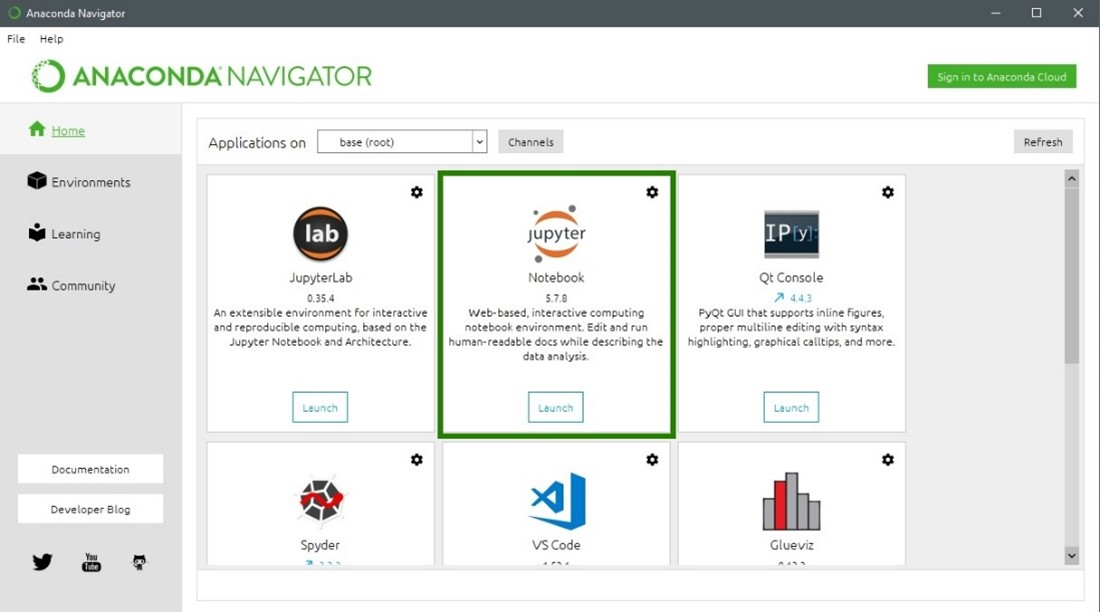
\includegraphics[width=1\textwidth]{images/anaconda.jpg}
\caption{\gls{anaconda} Navigator}
\label{fig:fig_01}
\end{figure}
\FloatBarrier

Theoretically, it would also have been possible for each developer to install \gls{anaconda} on their computer and work on the notebook, which is maintained on a Github repository. However, since the project is very hardware-heavy and compiling a machine learning model can take up to several hours, a \gls{virtual machine} turns out to be the better option.

\subsubsection{PyCharm}
is an integrated development environment (IDE) used for programming in the Python language, created by the Czech company JetBrains. I used it because it supports anaconda, git and as a debugger.
It natively supports jupyter notebooks is perfect because it is much more comfortable than jupyter itself, then it has several extensions that make programming easier and more intuitive.

\subsubsection{Github}
Provider with the function of hosting for software development and version control using Git.
Thanks to its free of charge nature it's used for most of the open-source projects.
That's why it's loved by the community of programmers, even I use it for this project to save files and use them from different locations.


\subsubsection{Overleaf}
Overleaf is cloud-based \LaTeX{} editor, which makes writing a scientific paper collaborative. \LaTeX{} is a software widely used in the academic world to create scientific texts, with useful formatting for mathematical, statistical, computer science, physics texts, which can be problematic on other text editors.
I preferred Overleaf to other solutions for the convenience, in fact there is no need to install anything, everything is accessible via the internet as with Colab.
Overleaf was useful for me to write this documentation, thanks also to its versioning nature.

\newpage
\section{The \gls{dataset}s}
Die Suche nach einem geeigneten Datensatz war nicht einfach und hat viel Zeit in Anspruch genommen. Wir haben das Internet nach Datensätzen, die speziell für Sentiment-Analysis geeignet sind, durchsucht. Dabei sind wir auf vielerlei Ergebnisse gestossen\cite{topDataset2020}, wobei die meisten Datensätze eine zu grosse Menge an Daten enthielten. Am Ende haben wir uns für ein \gls{dataset} mit Hotelbewertungen entschieden. Dieses eignet sich besonders, da eine Rezension zusätzlich mit einer numerischen Punktebewertung verknüpft ist, was es leichter macht, die Bewertung zu interpretieren.
\subsection{Hotel Review Description}
Das \gls{dataset} besteht aus ca. 515’000 Kundenbewertungen zu über 1493 Luxushotels innerhalb ganz Europa. Dabei ist jede Bewertung entweder als positiv oder negativ markiert. Das \gls{dataset} wird auf \gls{kaggle}\footnote{Siehe Referenzen für weitere Details \cite{515k_kaggle}} gehostet und wird von Jiashen Liu zur Verfügung gestellt.


\subsubsection*{Dataframe structure}
Die CSV-Datei enthält 17 Spalten, dies bedeutet, dass eine Kundenbewertung 17 Attribute enthält. In der Tabelle~\ref{tab:Dataframe structure} sind alle Attribute im Detail erklärt:

\begin{longtable}[ c ]{| m{5cm} | m{8cm}|}
\hline
\multicolumn{2}{|c|}{\textbf{Dataframe structure}}                                                                                                         \\ \hline
\endfirsthead
%
\multicolumn{2}{c}%
{{\bfseries  Tabelle \thetable\ Fortsetzung von vorheriger Seite}} \\
\hline
\multicolumn{2}{|c|}{\textbf{Dataframe structure}}                                                                                                         \\ \hline
\endhead
%
\textbf{Hotel\_Address  }                     & Adresse des Hotels.                                                                                  \\ \hline
\textbf{Review\_Date}                         & Datum an dem der Kunde seinen Kommentar   hinterlassen hat.                                          \\ \hline
\textbf{Average\_Score}                       & Durchschnittsbewertung. Berechnung durch alle   Kommentare des letzten Jahres.              \\ \hline
\textbf{Hotel\_Name}                          & Name des Hotels.                                                                                     \\ \hline
\textbf{Reviewer\_Nationality}                & Nationalität des Kunden.                                                                             \\ \hline
\textbf{Negative\_Review}                     & Negative Rezension des Kunden. Falls keine   negative Bewertung vorhanden ist, steht: “No Negative”. \\ \hline
\textbf{ReviewTotalNegativeWord Counts}        & Anzahl der Wörter in der negativen Rezension.                                                        \\ \hline
\textbf{Positive\_Review}                     & Positive Rezension des Kunden. Falls keine   positive Bewertung vorhanden ist, steht: “No Positive”. \\ \hline
\textbf{ReviewTotalPositiveWord Counts}        & Anzahl der Wörter in der positiven Rezension.                                                        \\ \hline
\textbf{Reviewer\_Score}                      & Punktzahlbewertung.                                                                                  \\ \hline
\textbf{TotalNumberofReviews ReviewerHasGiven} & Anzahl der Rezensionen, die der Kunde   insgesamt hinterlassen hat.                                  \\ \hline
\textbf{TotalNumberof\_Reviews}               & Anzahl der Bewertungen des Hotels.                                                                   \\ \hline
\textbf{Tags}                                 & Tags die der Kunde zur Rezension   hinterlassen hat.                                                 \\ \hline
\textbf{dayssincereview}                      & Anzahl Tage zwischen dem Bewertungsdatum und   Erstellen des \gls{dataset}s.                              \\ \hline
\textbf{AdditionalNumberof \_Scoring} & Die Anzahl der Bewertungen des Kunden, die nur aus   einer Punktebewertung bestehen und keinen Kommentar enthalten. \\ \hline
\textbf{lat}                                  & Breitengrad des Standorts des Hotels                                                                 \\ \hline
\textbf{lng}                                  & Längengrad des Standorts des Hotels                                                                  \\ \hline
\caption{Dataframe structure}
\label{tab:Dataframe structure}\\
\end{longtable}

\subsubsection*{Begründung der Auswahl}

Das \gls{dataset} bietet eine optimale Menge an Datensätzen für unser Projekt. Diese sind mit reichlich vielen Attributen versehen. Die Struktur der Datensätze ist sehr simpel und verständlich gehalten. Zudem hat \gls{kaggle} dieses \gls{dataset} mit einem Usability-Score von 8.2 bewertet.

\subsection{IMDB Review Description}
\subsubsection*{Dataframe structure}
\subsubsection*{Begründung der Auswahl}

\subsection{Amazon Maybe? Review Description}
\subsubsection*{Dataframe structure}
\subsubsection*{Begründung der Auswahl}
\newpage
\section{Verarbeiten des Datensatzes}

Im ersten Schritt werden alle Reviews (Positiv und Negativ) zusammengeführt.\\
Danach wird für jeden einzelnen Review ein neues Attribut "Review\_Type" erstellt, welches anhand des "Reviewer\_Score"-Attribut des Reviews bestimmt wird.

Der "Review\_Type" eines Reviews wird anhand folgender Kriterien bestimmt:

\begin{itemize}
\item \textbf{"awful"}: Reviewer\_Score bis 5.5
\item \textbf{"bad"}: Reviewer\_Score bis 7
\item \textbf{"good"}: Reviewer\_Score bis 8.7
\item \textbf{"great"}: Reviewer\_Score bis 9.7
\item \textbf{"excellent"}: Reviewer\_Score bis 10
\end{itemize}

Um unsere Daten in einen größeren Bereich von Bewertungen als nur "gut" oder "schlecht" einteilen zu können, haben wir mehrere Kategorien erstellt, wie in Bild~\ref{fig:fig_02} ersichtlich. Durch mehrere Tests haben wir festgestellt, dass die Anzahl der Bewertungen im Bereich "excellent" zu groß war, also haben wir ihn zwischen 9,7 und 10,0 begrenzt. Trotz der Begrenzung hat der Bereich "excellent" immer noch sehr viele Einträge.

\begin{figure}[H]
\centering
\includegraphics[width=1\textwidth]{images/2.jpg}
\caption{Anzahl der Bewertungen pro Kategorie}
\label{fig:fig_02}
\end{figure}
\FloatBarrier
\newpage
Damit wir unser Model später dazu trainieren können, User-Inputs in fünf verschiedene Kategorien einzuteilen, müssen für jede Kategorie gleich viele Testdaten zur Verfügung stehen. Aus diesem Grunde wurden unsere Daten so umgeformt, dass jede Kategorie nun die gleiche Anzahl ein Einträgen enthält, wie in Bild~\ref{fig:fig_03}.

\begin{figure}[H]
\centering
\includegraphics[width=1\textwidth]{images/3.jpg}
\caption{Einheitliche Grösse der Kategorien}
\label{fig:fig_03}
\end{figure}
\FloatBarrier

\section{Universal Sentence Encoder}	

Für unsere Arbeit wurde der multilingual sentence encoder von Tensorflow verwendet\footnote{ \url{https://tfhub.dev/google/universal-sentence-encoder-multilingual-large/3}}. Der Universal Sentence Encoder kodiert Text in hochdimensionale Vektoren, die für Textklassifikation, semantische Ähnlichkeit, Clustering und andere sprachbasierte Aufgaben verwendet werden können. Zudem ist er für Text mit einer Länge von mehr als einem Wort trainiert und optimiert, z. B. für Sätze, Phrasen oder kurze Paragraphen.

\newpage
\section{Preprocessing}
Das Preprocessing befasst sich damit, die Testdaten in die richtige Struktur und das richtige Format zu konvertieren, damit sie ein Machine Learning Model lesen kann.
Unsere Hotelreviews bestehen aus lesbaren Texten, sprich, String-Werten. Um diese jedoch in einem Machine Learning Model verwenden zu können, ist es notwendig, diese in numerische Vektoren zu transformieren.
In der SciKit-Lernbibliothek gibt es zwei Klassen, die für unseren Zweck geeignet sind: LabelEncoder und OneHotEncoder. Diese beiden Encoder sind Teil der \gls{Scikit-learn}-Bibliothek in Python und werden verwendet, um Textdaten in numerische Vektoren zu konvertieren, die für unser Model lesbar sind.
Zunächst einmal verwenden wir den OneHotEncoder. Hier stellt sich jedoch die Frage: wie funktioniert dieser Encoder?\\Zweck des OneHotEncoders ist es, Textwerte in Binärwerte umzuwandeln. Dabei wird jeder Text zuerst in Integerwerte umgewandelt, aus welchen dann die Binärwerte in form eines Vektors hergeleitet werden.
Danach, werden die Datensätze in Test- und Trainingssätze aufgeteilt. Dies ist eine grundlegende Operation des Machine Learnings.
Um die Aufteilung durchzuführen, verwenden wir die train\_test\_split Funktion, die in Bild~\ref{fig:fig_04} abgebildet ist:

\begin{figure}[ht!]
\centering
\includegraphics[width=0.5\textwidth]{images/4.jpg}
\caption{Aufteilung der Daten}
\label{fig:fig_04}
\end{figure}
\FloatBarrier

Danach werden die Datensätze, in Vektoren umgewandelt. In den Bildern~\ref{fig:fig_05} und~\ref{fig:fig_06} wird nochmals ersichtlich, wie lange dieser Prozess dauern kann.
\begin{figure}[ht!]
\centering
\includegraphics[width=0.7\textwidth]{images/5.jpg}
\caption{Umwandlung von Datensätzen in Vektoren}
\label{fig:fig_05}
\end{figure}
\FloatBarrier

\begin{figure}[ht!]
\centering
\includegraphics[width=0.7\textwidth]{images/8.jpg}
\caption{Daten-Training}
\label{fig:fig_06}
\end{figure}
\FloatBarrier

Nach dem Training des Train- und Test-Sets schauen wir uns die Struktur an, um zu sehen, ob die Daten richtig zugeordnet sind und die 5 Kategorien vorhanden sind.

\begin{figure}[ht!]
\centering
\includegraphics[width=0.5\textwidth]{images/10.jpg}
\caption{Dauer von Umwandlung von Datensätzen in Vektoren}
\label{fig:fig_07}
\end{figure}
\FloatBarrier

Wie auf Bild~\ref{fig:fig_07} zu erkennen ist, gibt es ca. 180'000 Trainingsdatensätze und 20'000 Testdatensätze. Diese zwei Sets sind wiederum in Input- und Output-Daten aufgeteilt. Die Input-Daten repräsentieren mögliche Benutzereingaben während die Output-Daten die zu erwartenden Sentiments darstellen.

\newpage
\section{Sentiment Analysis}
In diesem Kapitel werden wir genauer auf das Keras-Model eingehen, was es macht, wie es funktioniert und aufgebaut ist.
\subsection{Das \gls{keras}-Modell}
Das Model, welches Texte als Input nimmt und darauf eine Sentiment Analysis betreibt, besteht aus mehreren Schichten. Jede Schicht hat ihre eigene individuelle Aufgabe und übergibt ihre Resultate der nächsten Schicht. So werden Input-Daten eines Models von Schicht zu Schicht weiterverarbeitet, bis sie schlussendlich bei der untersten Schicht, den Output Neuronen, ankommen. Die einzelnen Schichten eines \gls{keras}-Models bestehen aus vielerlei Neuronen, deswegen ist ein \gls{keras}-Model auch unter dem Begriff “neuronales Netzwerk” bekannt. Das Model, welches im Projekt verwendet wurde, ist in Grafik~\ref{fig:fig_08} abgebildet.
\begin{figure}[ht!]
\centering
\includegraphics[width=0.8\textwidth]{images/6.jpg}
\caption{Das \gls{keras}-Model und dessen Schichten}
\label{fig:fig_08}
\end{figure}
\FloatBarrier

Dies Ziel eines Keras-Models ist es, dessen Neuronen solange anzupassen, bis diese Neuronen verschiedene Input-Werte möglichst nahe an das gewünschte Ergebnis verarbeiten können.

\subsubsection{Der Dense-Layer}
Der Dense-Layer ist einer der am meisten verwendeten Layer. Er zerlegt eine Datenmenge in eine bestimmte Anzahl von Neuronen. Diese Neuronen haben jeweils einen numerischen Wert zwischen 0 und 1. Ein Dense-Layer ist dementsprechenden eine Neuronen-basierte Repräsentation einer Datenmenge. Diese Neuronen dienen als Anhaltspunkt für die Verarbeitung nachfolgender Datenmengen. Demzufolge werden die Neuronen durchgehend angepasst durch sogenannte Aktivierungsfunktionen, bis sie die idealen Werte erreicht haben. Bei unserem Model ist die erste Schicht, die Input-Schicht, auf 256 Neuronen angesetzt und unsere Testdaten haben jeweils eine Arraylänge von 512 Einträgen, was bedeutet, dass je 2 Arraywerte auf 1 Neuron gemapt werden.

\subsubsection{Der Dropout-Layer}
Die Aufgabe des Dropout-Layers ist es, die Menge der Daten, die durch das Model fliessen zu reduzieren. Unser Model beginnt mit 256 Input-Neuronen und endet mit 5 Output-Neuronen. Um dies zu bewerkstelligen, ist es notwendig Datenflüsse nach und nach zusammenzuführen, aber auch loszuwerden, bis man schlussendlich bei 5 Output Neuronen ankommt.

\subsubsection{Kompilieren des Keras-Models}
Um das Keras Model nun laufen zu lassen, muss man es kompilieren und dabei die gewünschte Verlust- und Anpassungs-Funktion angeben, wie in Bild~\ref{fig:fig_09}.
\begin{figure}[ht!]
\centering
\includegraphics[width=0.7\textwidth]{images/11.jpg}
\caption{Kompilieren des Keras-Models}
\label{fig:fig_09}
\end{figure}
\FloatBarrier

Die angegebenen Parameter haben den folgenden Zweck:

\begin{itemize}
    \item Verlustfunktion - Hiermit wird gemessen, wie genau das Modell während des Trainings ist. Das Ergebnis dieser Funktions sollte mit der Zeit kleiner werden, um das Model in die richtige Richtung zu "steuern".
    \item Optimierer - Auf diese Weise wird das Model basierend auf den angezeigten Daten und seiner Verlustfunktion aktualisiert.
    \item Metriken - Dient zum Überwachen der Training- und Testschritte. Daraus lassen sich verschiedene Kenntnisse gewinnen. Im folgenden Beispiel wird die Genauigkeit verwendet.
\end{itemize}


\subsection{Erstellen einer Lernkurve}
Nach dem Ausführen eines Keras-Models, hat man die Option die Lernkurve des Models zu veranschaulichen mit der model.fit Funktion.
\begin{figure}[ht!]
\centering
\includegraphics[width=0.5\textwidth]{images/12.jpg}
\caption{History Erstellen mit Keras}
\label{fig:fig_10}
\end{figure}
\FloatBarrier

Für die Parameter der model.fit Methode in Bild~\ref{fig:fig_10} haben wir uns auf die Keras-Dokumentation und die Tutorials im Netz verlassen \cite{tutorial_keras}.\\
Die Parameter haben folgende Bedeutung:
\begin{itemize}
    \item X\_train, y\_train = Input Daten. X\_train sind Textwerte, y\_train die entsprechenden Sentiments.
    \item epochs = Integer. Anzahl der Epochen/Durchläufe zum Trainieren des Modells.
    \item verbose =  Grafische anzeige des Fortschritts (0, 1, oder 2). 0 = still, 1 = Fortschrittsbalken, 2 = eine Zeile pro Epoche.
    \item batch\_size = Integer oder None. Anzahl der Abtastungen pro Gradientenaktualisierung. Wenn nicht angegeben, wird batch\_size als Default auf 32 gesetzt.
    \item validation\_split = Float (Prozentsatz) zwischen 0 und 1. Teil der Trainingsdaten, der als Validierungsdaten verwendet werden soll. Das Model legt diesen Teil der Trainingsdaten beiseite und bewertet den Verlust und alle Model-Metriken auf diesen Daten am Ende jeder Epoche. 
    \item shuffle = Boolean. Ob die Trainingsdaten vor jeder Epoche gemischt werden sollen.
\end{itemize}
Die Keras Dokumentation ist unter folgendem Link \cite{keras} zu finden.

\subsection{Darstellung der Lernkurve}
Wenn der Validierungsverlust sinkt und die Validierungsgenauigkeit steigt, bedeutet dies, dass das Modell sich verbessert. Diese beiden Graphen~\ref{fig:fig_11} und~\ref{fig:fig_12} haben uns geholfen, die Funktionsweise unseres Models besser zu verstehen.

\begin{figure}[ht!]
\centering
\includegraphics[width=1\textwidth]{images/13.jpg}
\caption{Der Velauf der Fehlerrate}
\label{fig:fig_11}
\end{figure}
\FloatBarrier

\begin{figure}[ht!]
\centering
\includegraphics[width=1\textwidth]{images/14.jpg}
\caption{Die Entwicklung der Genauigkeit}
\label{fig:fig_12}
\end{figure}
\FloatBarrier
In diesem Fall ist ersichtlich, dass währenddem die Fehlerrate sinkt, die Genauigkeit steigt, dementsprechend lässt sich sagen, dass unser Model angemessen funktioniert.

\subsection{Das Auswerten des Models}

Mit der Funktion "evaluate" ist es möglich, die Genauigkeit des Models anhand einer Menge von Testdaten zu bestimmen. In der Variable "X\_test" sind die Textwerte der Testdaten vorhanden und in "y\_test" die Lösungen, bzw. die entsprechenden Sentiments der Textwerte. Das Model geht dann durch alle Textwerte der Testdaten durch, berechnet das Sentiment, und vergleicht jeweils das errechnete Sentiment mit dem Resultat des Testdatensatzes.
Im Bild~\ref{fig:fig_13} ist ersichtlich, dass das Model eine accuracy von 0.4844 erreicht hat. Dies liegt daran, dass das Model auf dem Bild aus Zeitgründen mit sehr wenigen Testdaten erstellt wurde. Danach fügen wir denselben Text in das Model hinein und sehen, dass das Resultat mit der Lösung des Datensatzes übereinstimmt.
\begin{figure}[ht!]
\centering
\includegraphics[width=1\textwidth]{images/15.jpg}
\caption{Genauigkeit des Models auswerten}
\label{fig:fig_13}
\end{figure}
\FloatBarrier

\newpage
\section{Das Testen des Models}

Jetzt ist das Model bereit mit den Testdatensätzen und weiteren Benutzereingaben getestet zu werden. Bei den Testdatensätzen ist jeweils ein Text und das zu erwartende Gefühls-Resultat enthalten. Beim Testen eines Testdatensatzes sollte also das Resultat des Models mit dem Resultat des jeweiligen Testdatensatzes übereinstimmen. Wie in den Bildern~\ref{fig:fig_14} und~\ref{fig:fig_15} zu sehen ist, geben wir jeweils zuerst einen Text und dessen zu erwartende Bewertung aus bei "Prediction X text and rating". Danach fügen wir diesen Text in das Model ein und vergleichen die Ausgabe des Modells mit der Lösung.\\Wenn das Model korrekt funktioniert, sollten die beiden Ergebnisse von "Prediction X text and rating" und "Prediction X result" übereinstimmen.

\begin{figure}[ht!]
\centering
\includegraphics[width=1\textwidth]{images/16.jpg}
\caption{Erste Vorhersage}
\label{fig:fig_14}
\end{figure}
\FloatBarrier

\begin{figure}[ht!]
\centering
\includegraphics[width=1\textwidth]{images/17.jpg}
\caption{Zweite Vorhersage}
\label{fig:fig_15}
\end{figure}
\FloatBarrier

Des Weiteren ist es nun auch möglich, das Model mit beliebigen Benutzereingaben zu testen. In Bild~\ref{fig:fig_16} sind ein paar Beispiele zu sehen. Wie man sieht, scheint das Model einigermassen korrekte Sentiments abzugeben.

\begin{figure}[ht!]
\centering
\includegraphics[width=1\textwidth]{images/18.jpg}
\caption{Testen des Models mit Benutzereingaben}
\label{fig:fig_16}
\end{figure}
\FloatBarrier

\section{Herausforderungen}
In diesem Abschnitt befassen wir uns mit den Herausforderungen, die sich während der Arbeit am Projekt herausgestellt haben, und wir diese behandelt haben.

\subsubsection*{Finden des geeigneten \gls{dataset}s} 
Unser erstes Problem war es, einen passenden Datensatz für unsere Bedürfnisse zu finden. Um ein Modell zu trainieren, brauchten wir einen Datensatz, der für die Sentiment-Analyse relevant, aber auch gross genug war, um ihn in Trainings- und Test-Sets aufzuteilen, ohne die Modellqualität zu verlieren. Zu unseren Gunsten hat Kaggle reichlich viele Beispiele von guten Datensätzen.

\subsubsection*{\gls{virtual machine}}
Unser zweites Problem bezieht sich auf unsere virtuelle Maschine. Diese war anfangs hardware-technisch nicht zureichend für unser Projekt ausgestattet, da unser Projekt sehr rechenintensive Programme verwendet. Nach Anfrage auf eine leistungsstärkere Maschine wurde dieses Problem gelöst. In der Zwischenzeit, sind wir wieder zu Google \gls{colab} umgezogen, dort waren bereits viele Abhängigkeiten installiert.

\subsubsection*{Google \gls{colab}}
Ein Problem, das wir mit \gls{colab} hatten, war, dass wir jedes Mal, wenn wir das Notebook öffneten, das \gls{dataset} neu importieren mussten. Dies nam jeweils eine grosse Menge an Zeit in Anspruch, da unser \gls{dataset} sehr gross ist. Wir haben auch versucht, \gls{colab} auf der virtuellen Maschine laufen zu lassen, aber \gls{colab} stoppt automatisch nach einer bestimmten Zeit die Ausführung, was nicht ideal für unsere Arbeit war, da das Trainieren eines Modells bis zu mehreren Stunden andauern kann. Letzten Endes stellte sich Anaconda als die geeignete Lösung hervor.

\subsubsection*{\gls{anaconda} und \gls{jupyter}}
Beim Übergang von \gls{colab} auf die \gls{virtual machine}, haben wir bei \gls{colab} eine Datei mit allen benötigten Libraries exportiert. Daraus haben wir auf der virtuellen Maschine mit \gls{anaconda} versucht, eine neue Umgebung zu erstellen, die alle Libraries von \gls{colab} enthält. Jedoch schlug die Ausführung mit \gls{anaconda} fehl, aufgrund eines Versionskonfliktes zwischen den Libraries. Womöglich hatte dieser Fehler einen Zusammenhang mit fehlenden Zugriffsrechten in der Systemadministration. Dementsprechend verwarfen wir die Idee eine neue Umgebung zu erstellen und arbeiteten auf der Standardumgebung von \gls{anaconda}, auf der alles ohne Probleme verlief.

\subsubsection*{Grosse Verarbeitungszeiten}
Sowohl auf \gls{colab} als auch lokal auf der virtuellen Maschine mit \gls{anaconda} ist die Verarbeitungsdauer der Datensätze mit dem Sentence Encoder mehrere Stunden lang. Um lange Wartezeiten zu umgehen, haben wir des Öfteren mit verkürzten Versionen unseres \gls{dataset}s gearbeitet. Für das finale Produkt, ist jedoch eine grosse Anzahl an Daten erforderlich, weshalb wir gegen Ende des Projektes unser Sentiment-Analysis-Model nochmals mit der ganzen Menge an Daten gefüttert haben.
\newpage
\section{Conclusion Schlussstand des Projekts}
Im jetzigen Zustand haben wir ein funktionierendes Sentiment-Analysis-Model, welches einen Text lesen und ein Sentiment dazu abgeben kann, welches sich in einem Rahmen von 5 verschiedenen Kategorien befindet. Die Genauigkeit, oder die Wahrscheinlichkeit die richtige Kategorie zu treffen, liegt dabei bei rund 60\%. Das Model ist dazu trainiert ganze Sätze zu verarbeiten. Bei einzelnen Worten könnte es deshalb etwas willkürliche Resultate ausgeben. Momentan ist das Model noch an ein Jupyter-Notebook gebunden, im nächsten Schritt jedoch, würde man dieses Model exportieren und in eine serverseitige Applikation einbinden, welche sich beispielsweise über eine API aufrufen lässt.

\section{Attachments}
In addition to the documentation, the following documents are available:
\begin{itemize}
    \item \textbf{"GefuehleModellierenNLP.html"}, der Source Code des Projekts im html-Format
    \item \textbf{"GefuehleModellierenNLP.pdf"}, der Source Code des Projekts im pdf-Format
    \item \textbf{"GefuehleModellierenZeitplan.pdf"}, der Zeitplan des Projekts im pdf-Format
    \item \textbf{"GefuehleModellierenZeitplan.xlsx"}, der Zeitplan des Projekts im excel-Format
    \item \textbf{"Arbeitsaufteilungein.docx"}, die Word-Datei für die Unterteilung der Kapitel
\end{itemize}




